\graphicspath{{./figures}}

\section{Software}

\subsection{Classes}
The Arduino framework will be used, as well as a custom C++ library for re-usability across GS and PQ code. Tables \ref{tab:gpsUML} to \ref{tab:groundStationUML} in the Appendix describe expected class functionality.

Although the CSP protocol was considered, it was decided to rather develop a simple ASCII protocol between the PQ and GS. This flow control is encapsulated in the \textit{link} class. The link object can be set to either \textit{Controller} or \textit{Responder} mode for the GS and PQ respectively, and allows \textit{Telemetry} and \textit{Telecommand} operating modes. In \textit{Telemetry} mode, the responder sends data at regular intervals to the controller, pausing at longer intervals to \textit{listen} for a ``telecommand mode" message. If the responder receives this message, it sends an ``ACK" message, and switches to \textit{Telecommand} mode to await further commands.

The \textit{PqTnc} and \textit{PqUnit} classes where designed as Singleton classes for the GS and PQ respectively. Here, the GS is referred to as a \textit{Terminal Node Controller} (TNC) with reference to the serial interface it exposes to a host computer. This is summarised in the created \textit{SUNCQ} protocol in Appendix \ref{sec:appendix_suncq}.

\subsection{Tracking}
For path tracking, it is decided to store data in the TNC object on the ESP32 itself, instead of streaming it from the host computer. This is so that the host can be disconnected, and the payload will still be tracked.

An "instant" is defined as both a location and a time. The PqTnc object performs a check in its update loop to determine if an instant has been reached, based on its GPS received time. The GroundStation object should store two locations - the previous location in the path, and the location it is moving towards. The mount is pointed at the location which linearly interpolates its these two instants, with a factor based on the current time, and the time of the two instants.

To allow direct GPS tracking and flight path tracking to be used simultaneously, it was decided to follow the flight path data until a location from the satellite is received. When a "known" location is received, it is used for a specified timeout "trust" period, until a new location is received and is overwritten. A pseudo low-pass filter is added to the ground station to prevent pointing "jitter". The final algorithm is shown in Figure \ref{fig:trackingAlgorithm}.

\begin{figure}[!htb]
  \centering
  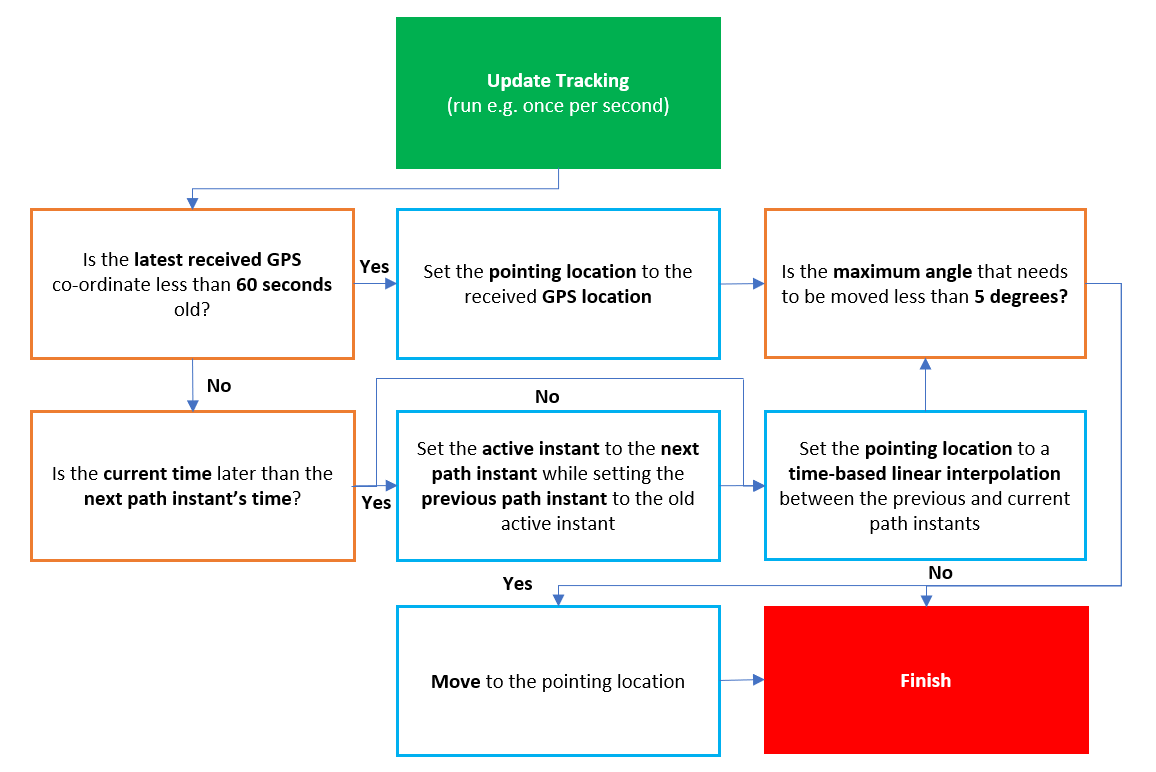
\includegraphics[width=0.95\textwidth]{trackingAlgorithm}
  \caption{Tracking Algorithm Flow Diagram}
  \label{fig:trackingAlgorithm}
\end{figure}